\documentclass[]{article}
\usepackage{lmodern}
\usepackage{amssymb,amsmath}
\usepackage{ifxetex,ifluatex}
\usepackage{fixltx2e} % provides \textsubscript
\ifnum 0\ifxetex 1\fi\ifluatex 1\fi=0 % if pdftex
  \usepackage[T1]{fontenc}
  \usepackage[utf8]{inputenc}
\else % if luatex or xelatex
  \ifxetex
    \usepackage{mathspec}
  \else
    \usepackage{fontspec}
  \fi
  \defaultfontfeatures{Ligatures=TeX,Scale=MatchLowercase}
\fi
% use upquote if available, for straight quotes in verbatim environments
\IfFileExists{upquote.sty}{\usepackage{upquote}}{}
% use microtype if available
\IfFileExists{microtype.sty}{%
\usepackage{microtype}
\UseMicrotypeSet[protrusion]{basicmath} % disable protrusion for tt fonts
}{}
\usepackage[margin=1in]{geometry}
\usepackage{hyperref}
\hypersetup{unicode=true,
            pdftitle={Latex Table in R Markdown},
            pdfborder={0 0 0},
            breaklinks=true}
\urlstyle{same}  % don't use monospace font for urls
\usepackage{graphicx,grffile}
\makeatletter
\def\maxwidth{\ifdim\Gin@nat@width>\linewidth\linewidth\else\Gin@nat@width\fi}
\def\maxheight{\ifdim\Gin@nat@height>\textheight\textheight\else\Gin@nat@height\fi}
\makeatother
% Scale images if necessary, so that they will not overflow the page
% margins by default, and it is still possible to overwrite the defaults
% using explicit options in \includegraphics[width, height, ...]{}
\setkeys{Gin}{width=\maxwidth,height=\maxheight,keepaspectratio}
\IfFileExists{parskip.sty}{%
\usepackage{parskip}
}{% else
\setlength{\parindent}{0pt}
\setlength{\parskip}{6pt plus 2pt minus 1pt}
}
\setlength{\emergencystretch}{3em}  % prevent overfull lines
\providecommand{\tightlist}{%
  \setlength{\itemsep}{0pt}\setlength{\parskip}{0pt}}
\setcounter{secnumdepth}{0}
% Redefines (sub)paragraphs to behave more like sections
\ifx\paragraph\undefined\else
\let\oldparagraph\paragraph
\renewcommand{\paragraph}[1]{\oldparagraph{#1}\mbox{}}
\fi
\ifx\subparagraph\undefined\else
\let\oldsubparagraph\subparagraph
\renewcommand{\subparagraph}[1]{\oldsubparagraph{#1}\mbox{}}
\fi

%%% Use protect on footnotes to avoid problems with footnotes in titles
\let\rmarkdownfootnote\footnote%
\def\footnote{\protect\rmarkdownfootnote}

%%% Change title format to be more compact
\usepackage{titling}

% Create subtitle command for use in maketitle
\newcommand{\subtitle}[1]{
  \posttitle{
    \begin{center}\large#1\end{center}
    }
}

\setlength{\droptitle}{-2em}

  \title{Latex Table in R Markdown}
    \pretitle{\vspace{\droptitle}\centering\huge}
  \posttitle{\par}
    \author{}
    \preauthor{}\postauthor{}
    \date{}
    \predate{}\postdate{}
  
\usepackage{array}
\usepackage{fontspec}
\usepackage{hyperref}
\usepackage[labelformat=empty]{caption}

\begin{document}
\maketitle

first \newline

\renewcommand{\arraystretch}{2}

\begin{table}
\caption{
Article ID 1 : \textit{(Scolforo, McTague, Raimundo, et al., 2018)}\\
}
\begin{tabular}{p{0.2\textwidth} p{0.8\textwidth}}
\hline
Student & NA \\ \hline
Title.student & Comparison of taper functions applied to eucalypts of varying genetics in Brazil: Application and evaluation of the penalized mixed spline approach \\ \hline
Authors.student & Scolforo, H.F., McTague, J.P., Raimundo, M.R., Weiskittel, A., Carrero, O., Scolforo, J.R.S. \\ \hline
Year.student & 2017 \\ \hline
Species & Eucalypts \\ \hline
Base.URL & \url{http://www.nrcresearchpress.com/doi/10.1139/cjfr-2017-0366#.W2Sb6Lhx02w} \\ \hline
Paper.local.file & NA \\ \hline
Equations & NA \\ \hline
\end{tabular}\end{table}

\begin{table}
\caption{
Article ID 3 : \textit{(Tang, Pérez-Cruzado, Fehrmann, et al., 2016)}\\
}
\begin{tabular}{p{0.2\textwidth} p{0.8\textwidth}}
\hline
Student & NA \\ \hline
Title.student & Development of a Compatible Taper Function and Stand-Level Merchantable Volume Model for Chinese Fir Plantations \\ \hline
Authors.student & Xiaolu Tang,César Pérez-Cruzado,Lutz Fehrmann,Juan Gabriel Álvarez-González,Yuanchang Lu,and Christoph Kleinn, \\ \hline
Year.student & 2016 \\ \hline
Species & Cunninghamia lanceolata [Lamb.] Hook \\ \hline
Base.URL & \url{https://www.ncbi.nlm.nih.gov/pubmed/26799399} \\ \hline
Paper.local.file & pone.0147610.pdf \\ \hline
Equations & 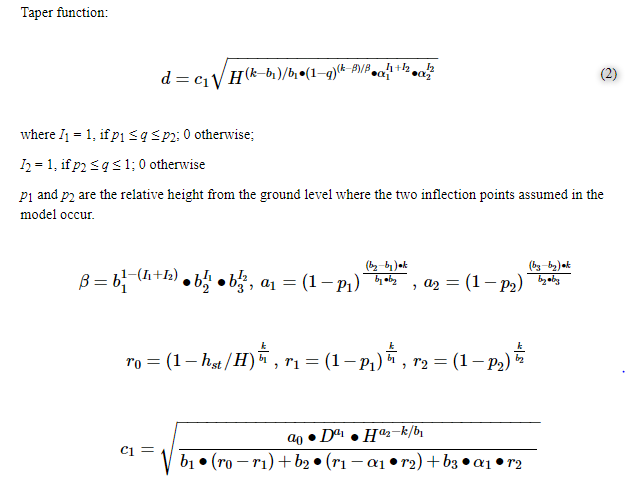
\includegraphics[width=0.8\textwidth]{Equations/2016TangEtAl.png} \\ \hline
\end{tabular}\end{table}

\begin{table}
\caption{
Article ID 8 : \textit{(Arnoni Costa, Guimarães Finger, Schneider, et al., 2016)}\\
}
\begin{tabular}{p{0.2\textwidth} p{0.8\textwidth}}
\hline
Student & NA \\ \hline
Title.student & Taper function and timber assortments for Araucaria angustifolia \\ \hline
Authors.student & Emanuel Arnoni Costa, César Augusto Guimarães Finger, Paulo Renato Schneider, André Felipe Hess \\ \hline
Year.student & 2016 \\ \hline
Species & Araucaria angustifolia \\ \hline
Base.URL & \url{http://www.redalyc.org/articulo.oa?id=53446151016} \\ \hline
Paper.local.file & 53446151016.pdf \\ \hline
Equations & NA \\ \hline
\end{tabular}\end{table}

\begin{table}
\caption{
Article ID 10 : \textit{(Arias-Rodil, Castedo-Dorado, Cámara-Obregón, et al., 2015)}\\
}
\begin{tabular}{p{0.2\textwidth} p{0.8\textwidth}}
\hline
Student & NA \\ \hline
Title.student & Fitting and Calibrating a Multilevel Mixed-Effects Stem Taper Model for Maritime Pine in NW Spain \\ \hline
Authors.student & Manuel Arias-Rodil, Fernando Castedo-Dorado, Asunción Cámara-Obregón, Ulises Diéguez-Aranda \\ \hline
Year.student & 2015 \\ \hline
Species & Pinus pinaster Ait. \\ \hline
Base.URL & \url{http://europepmc.org/backend/ptpmcrender.fcgi?accid=PMC4668033&blobtype=pdf} \\ \hline
Paper.local.file & pone.0143521.pdf \\ \hline
Equations & NA \\ \hline
\end{tabular}\end{table}

\begin{table}
\caption{
Article ID 11 : \textit{(Rodríguez, Lizarralde, and Bravo, 2015)}\\
}
\begin{tabular}{p{0.2\textwidth} p{0.8\textwidth}}
\hline
Student & NA \\ \hline
Title.student & Comparison of stem taper equations for eight major tree species in the Spanish Plateau \\ \hline
Authors.student & Francisco Rodríguez1, Iñigo Lizarralde1 and Felipe Bravo \\ \hline
Year.student & 2015 \\ \hline
Species & Various \\ \hline
Base.URL & \url{http://revistas.inia.es/index.php/fs/article/view/6229} \\ \hline
Paper.local.file & 6229-27194-1-PB.pdf \\ \hline
Equations & NA \\ \hline
\end{tabular}\end{table}

\begin{table}
\caption{
Article ID 12 : \textit{(Návar, Rodríguez-Flores, and Domínguez-Calleros, 2013)}\\
}
\begin{tabular}{p{0.2\textwidth} p{0.8\textwidth}}
\hline
Student & NA \\ \hline
Title.student & Taper functions and merchantable timber for temperate forests of northern Mexico \\ \hline
Authors.student & J. Návar, F. de Jesús Rodríguez-Flores, P.A. Domínguez-Calleros \\ \hline
Year.student & 2013 \\ \hline
Species & P.pseudostrobus, P. hartwegii, P. cooperi, P. ayacahuite, Q. spp, P. durangensis, P. leiophylla, P. teocote, P. arizonica, Quercus spp \\ \hline
Base.URL & \url{http://www.editurasilvica.ro/afr/56/1/navar.pdf} \\ \hline
Paper.local.file & navar.pdf \\ \hline
Equations & NA \\ \hline
\end{tabular}\end{table}

\begin{table}
\caption{
Article ID 13 : \textit{(Özçelik and Dirican, 2017)}\\
}
\begin{tabular}{p{0.2\textwidth} p{0.8\textwidth}}
\hline
Student & NA \\ \hline
Title.student & Individual taper models for natural cedar and Taurus fir mixed stands of Bucak Region, Turkey \\ \hline
Authors.student & Ramazan Özçelik, Osman Dirican \\ \hline
Year.student & 2017 \\ \hline
Species & Cedrus libani A. Rich., Abies cilicica Carr. \\ \hline
Base.URL & \url{http://dergipark.gov.tr/download/article-file/330518} \\ \hline
Paper.local.file & 10.17099-jffiu.290845-330518.pdf \\ \hline
Equations & NA \\ \hline
\end{tabular}\end{table}

\begin{table}
\caption{
Article ID 14 : \textit{(Machado, Urbano, and Conceiç{ã}o, 2005)}\\
}
\begin{tabular}{p{0.2\textwidth} p{0.8\textwidth}}
\hline
Student & NA \\ \hline
Title.student & Comparação de Métodos de Estimativa de Volume para Pinus oocarpa em Diferentes Idades e Diferentes Regimes de Desbastes \\ \hline
Authors.student & Sebastião do Amaral Machado, Edilson Urbano, Marcio Barbosa da Conceição \\ \hline
Year.student & 2005 \\ \hline
Species & Pinus oocarpa \\ \hline
Base.URL & \url{https://pfb.cnpf.embrapa.br/pfb/index.php/pfb/article/view/242/193} \\ \hline
Paper.local.file & 242-1027-1-PB.pdf \\ \hline
Equations & NA \\ \hline
\end{tabular}\end{table}


\end{document}
